%% Figure 1: overview of the VALID-Aug probe (TikZ). Compile:  pdflatex Figure_1.tex
\documentclass[tikz,border=2pt]{standalone}
\usepackage[T1]{fontenc}
\usepackage{lmodern}
\usepackage{amsmath,amssymb}
\usetikzlibrary{arrows.meta,positioning}
\begin{document}
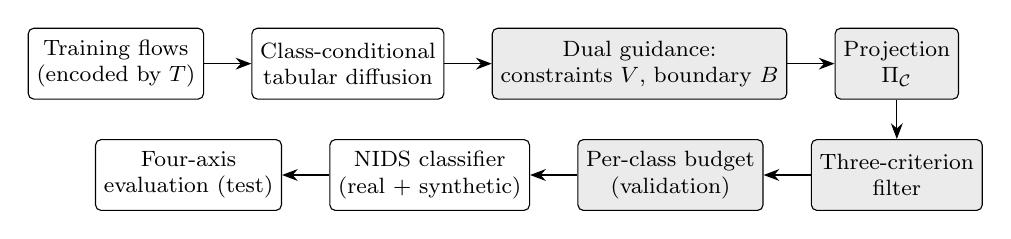
\begin{tikzpicture}[node distance=5mm and 6mm,
  box/.style={draw,rounded corners=2pt,align=center,font=\footnotesize,minimum height=9mm,inner sep=3pt},
  new/.style={box,fill=black!8},>={Stealth[length=2mm]}]
\node[box] (data) {Training flows\\(encoded by $T$)};
\node[box,right=of data] (diff) {Class-conditional\\tabular diffusion};
\node[new,right=of diff] (guide) {Dual guidance:\\constraints $V$, boundary $B$};
\node[new,right=of guide] (proj) {Projection\\$\Pi_{\mathcal{C}}$};
\node[new,below=of proj] (filter) {Three-criterion\\filter};
\node[new,left=of filter] (budget) {Per-class budget\\(validation)};
\node[box,left=of budget] (clf) {NIDS classifier\\(real + synthetic)};
\node[box,left=of clf] (eval) {Four-axis\\evaluation (test)};
\draw[->] (data)--(diff); \draw[->] (diff)--(guide); \draw[->] (guide)--(proj);
\draw[->] (proj)--(filter); \draw[->] (filter)--(budget); \draw[->] (budget)--(clf); \draw[->] (clf)--(eval);
\end{tikzpicture}
\end{document}
